\section{Tiến hóa vi phân (Differential Evolution)} % (fold)
\label{sec:Tiến hóa vi phân (Differential Evolution)}

\subsection{Giới thiệu và thuật toán chung} % (fold)
\label{sub:Giới thiệu và thuật toán chung}

\begin{frame}{Giới thiệu chung}
  \textbf{Differential Evolution} (DE) là một giải thuật tiến hóa tương đối nổi
  tiếng sau giải thuật di truyền (GA). Được lần đầu công bố lần đầu bởi R. Storn
  và K. Price vào năm 1995, giải thuật được ứng dụng rộng rãi trong việc giải
  các bài toán tối ưu phi tuyến.

  DE được cài đặt đơn giản hơn GA, nhưng ý tưởng của nó không được tự nhiên
  bằng. Dù vậy, DE, trong nhiều trường hợp, có thể đưa ra những kết quả tốt hơn
  GA và các giải thuật di truyền khác. Tính đơn giản của DE cũng làm cho thuật
  toán này dễ dàng được ứng dụng và mở rộng. Tuy nhiên, DE chỉ có thể được áp
  dụng để giải các bài toán tối ưu liên tục.

  Thuật ngữ \textit{Differential} có thể được dịch thành \textit{vi phân}, nhưng
  thực chất thuật toán không sử dụng đạo hàm. Từ này nên hiểu theo nghĩa là sự
  chênh lệch và sai khác (giống chữ \textit{difference}) giữa các cá thể.
  Lượng chênh lệch này sẽ được sử dụng để thực hiện đột biến các cá thể trong giải
  thuật.
\end{frame}

\begin{frame}[fragile]
\frametitle{Thuật toán chung}
  DE sử dụng các toán tử lai ghép, đột biến và chọn lọc giống như GA. Tuy nhiên
  toán tử chọn lọc được định sẵn: cá thể con chỉ được thêm vào quần thể nếu nó
  tốt hơn cá thể cha mẹ của nó.
  \begin{minted}[fontsize=\footnotesize]{python}
def de():
  population = init_pop()
  while True:
    # lặp với mọi cá thể trong quần thể
    for parent in population:
      # tạo một cá thể đột biến từ các cá thể khác trong quần thể
      mutant = new_mutant(population, parent)
      # thực hiện lai ghép giữa cá thể đột biến và cá thể gốc
      offspring = crossover(parent, mutant)
      if fitness(mutant) > fitness(parent):
        # nếu cá thể con tốt hơn cá thể gốc,
        # cá thể con sẽ thay thế cá thể gốc trong quần thể
        population[population.index(parent)] = offspring
    yield population
\end{minted}
\end{frame}

% subsection Giới thiệu và thuật toán chung (end)

\subsection{Toán tử lai ghép và đột biến trong DE} % (fold)
\label{sub:Toán tử lai ghép và đột biến trong DE}

\begin{frame}{Toán tử lai ghép trong DE}
Về mặt lý thuyết, mọi toán tử lai ghép ứng dụng được cho các mảng số thực đều có
thể sử dụng được cho DE. Tuy nhiên trong thực tế, DE thường chỉ sử dụng một
trong hai loại lai ghép sau:
\begin{itemize}
\item Lai ghép nhị thức (Binomial Crossover) có thể coi là một biến dạng của Uniform
  Crossover. Mỗi gen của cá thể con sẽ được cho là gen tương ứng của cá thể gốc
  hoặc của cá thể đột biến tùy theo giá trị của một biến ngẫu nhiên:
  \[
    offspring_{i} = \begin{cases}
      mutant_{i}, &\text{ nếu } \operatorname{rand}() < CR\\
      parent_{i}, &\text{ nếu ngược lại }
      
    \end{cases}
  .\] 

  Ở đây, tham số \( CR \in [0, 1] \) (crossover rate, tỉ lệ lai ghép), ảnh hưởng
  trực tiếp đến việc chọn gen từ cá thể nào. \( CR \) càng gần \( 1 \), thì cá
  thể con càng giống như cá thể gốc.
\end{itemize}
\end{frame}

\begin{frame}{Toán tử lai ghép trong DE}
Cách làm này có thể sinh ra những cá thể con giống y hệt cá thể gốc, đặc biệt
nếu \( CR \) gần với \( 1 \). Khi đó, cá thể con chắc chắn sẽ không được lựa
chọn vào thay cho cá thể gốc, nên ta nên tránh trường hợp này xảy ra bằng cách
ép cá thể con lấy ít nhất một gen từ cá thể đột biến:
  \[
    offspring_{i} = \begin{cases}
      mutant_{i}, &\text{ nếu } \operatorname{rand}() < CR \text{ hoặc } i = R\\
      parent_{i}, &\text{ nếu ngược lại }
      
    \end{cases}
  ,\] 
  trong đó \( R \) là một chỉ số cố định cho mọi chỉ số \( i \), được chọn ngẫu
  nhiên khi bắt đầu lai ghép.
\end{frame}

\begin{frame}{Toán tử lai ghép trong DE}
\begin{itemize}
\item Toán tử lai ghép mũ (Exponential Crossover) là một toán tử có nguồn gốc từ
  Two-point Crossover. Cụ thể hơn, ta sẽ thay thế một đoạn trên cá thể gốc
  bởi đoạn tương ứng trên cá thể đột biến để thu được cá thể con.

  Điểm khác biệt giữa toán tử này với Two-point Crossover là đoạn thay thế này
  có thể "tràn" modulo, trở thành hai đoạn con ở đầu và cuối nhiễm sắc
  thể.
\end{itemize}
  \begin{figure}
    \centering
    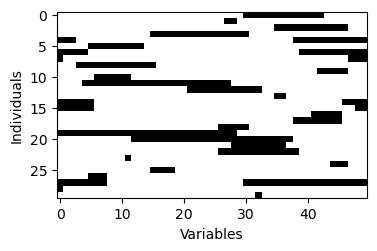
\includegraphics[height=0.5\textheight]{res/xx.png}
    \caption{Các cá thể con sinh ra từ Exponential Crossover}
  \end{figure}
\end{frame}

\begin{frame}{Toán tử đột biến trong DE}
  Toán tử đột biến chính là điểm đặc trưng lớn nhất của DE. Như cái tên của
  thuật toán, ta sẽ thực hiện đột biến bằng các giá trị chênh lệch giữa các
  vector cá thể.

  Ý tưởng chung của toán tử đột biến là ta chọn ra một cá thể cơ sở \( b \) (base) và
  một nhóm các cá thể \( G = \{g_{1}, g_{2}, \ldots , g_{|G|}\}  \). Căn cứ vào
  độ chênh lệch \( \operatorname{diff}(G) \) giữa các cá thể trong \( G \), ta
  cộng thêm một lượng vào vector \( b \) để thu được cá thể đột biến:
  \[
    mutant = b + F \cdot \operatorname{diff}(G)
  .\] 
  Để sử dụng nhiều thông tin từ quần thể, ta chọn các cá thể \( b, g_{1}, g_{2},
  \ldots , g_{|G|} \) phân biệt và khác với cá thể gốc \( parent \).

  \( F \) là một tham số được nhân vào độ chênh lệch để thu được vector được
  thêm vào cá thể cơ sở.
\end{frame}

\begin{frame}{Toán tử đột biến trong DE}
  Trong trường hợp đơn giản nhất, ta lấy nhóm \( G \) có hai phần tử: \( G =
  \{g_{1}, g_{2}\}   \). Khi đó, hàm độ chênh lệch tự nhiên nhất là hiệu của 2
  vector này:
  \begin{align*}
    \operatorname{diff}(G) &=  g_{2} - g_{1}\\ 
    \implies mutant &= b + F(g_{2} - g_{1})
  .\end{align*}
  Tham số \( F \) ở đây sẽ được chọn bằng một số thực trong đoạn \( [0, 2] \).
  \begin{figure}
    \centering
    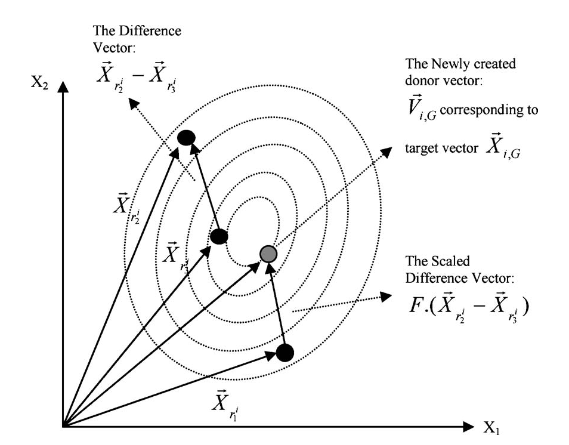
\includegraphics[height=0.4\textheight]{res/de2d.png}
    \caption{Minh họa cho phép đột biến của DE trong 2 chiều}
  \end{figure}
\end{frame}

\begin{frame}{Toán tử đột biến trong DE}
  Ta có thể thiết lập các toán tử đột biến phức tạp hơn một cách tương tự. Chẳng
  hạn, ta có thể lấy nhóm \( G = \{g_{1}, g_{2}, g_{3},
  g_{4}\}   \) là 2 cặp cá thể:
  \[
    \operatorname{diff}(G) = (g_{2} - g_{1}) + (g_{4} - g_{3})
  .\] 
  Thậm chí, ta có thể sử dụng phép nhân ma trận để có những toán tử đột biến
  linh hoạt hơn nữa:
  \begin{align*}
    \operatorname{diff}(G) &= \begin{bmatrix} g_{2} - g_{1} \\ g_{4} - g_{3}
    \end{bmatrix}\\
      \implies mutant &= b + F \cdot \operatorname{diff} (G) \\
                      &= b + \begin{bmatrix} F_{1} & F_{2} \end{bmatrix}
                      \begin{bmatrix} g_{2} - g_{1} \\ g_{4} - g_{3}
                      \end{bmatrix}  \\
                      &= b + F_{1}(g_{2} - g_{1}) + F_{2}(g_{4} - g_{3}) \\
  .\end{align*}
\end{frame}

\begin{frame}{Toán tử đột biến trong DE}
  Ngoài ra, cách chọn các cá thể \( b \) và nhóm cá thể \( G \) cũng vô cùng
  phong phú. Ta có thể dùng các toán tử chọn lọc hoặc chỉ đơn giản là chọn các
  cá thể ngẫu nhiên từ quần thể.

  Một lớp các toán tử đột biến của DE được có tên chuẩn là DE/x/y,
  trong đó:
\begin{itemize}
\item x: mô tả cách chọn cá thể cơ sở \( b \): \texttt{best} là chọn cá thể tốt
  nhất, \texttt{rand} là chọn cá thể ngẫu nhiên.
\item y: số cặp phần tử tính chênh lệch trong \( G \):
  \begin{align*}
    G &= \{g_{1}, g_{2}, \ldots , g_{2y}\}  \\
    \operatorname{diff}(G) &= \sum_{k = 1}^{y} (g_{2k} - g_{2k - 1})
  .\end{align*}
\end{itemize}
\end{frame}

\begin{frame}{Toán tử đột biến trong DE}
  Chẳng hạn, ta có các toán tử đột biến thông dụng sau:
\begin{itemize}
  \item DE/rand/1: \( mutant = b_{rand} + F(g_{2} - g_{1}) \).
\item DE/best/1: \( mutant = b_{best} + F(g_{2} - g_{1}) \).
\item DE/best/2: \( mutant = b_{best} + F(g_{2} - g_{1}) + F(g_{4} - g_{3}) \).
\item DE/target-to-best/1: \( mutant = b_{rand} + F(b_{best} - b_{rand}) +
  F(g_{2} - g_{1}) \).
\end{itemize}

Trong đó, toán tử thông dụng nhất là DE/rand/1.

\end{frame}
% subsection Toán tử lai ghép và đột biến trong DE (end)

\begin{frame}{Contour Matching}
  K. Price \textit{et al.} tìm ra một tính chất của các phép đột biến này, gọi là
  \textbf{Contour Matching}, để giải thích tính ưu việt của thuật toán DE.

  Contour Matching là hiện tượng xảy ra trong DE khi quần thể thich nghi theo
  hàm fitness dẫn đến những khu vực tiềm năng sẽ được khám phá ngay khi chúng
  được tìm ra. Các vector chênh lệch tính toán như trên thỏa mãn tính chất này,
  cả về mặt độ lớn lẫn hướng.

  Chẳng hạn, khi quần thể tiến hóa gồm hai nhóm đang tiếp cận đến hai điểm tối
  ưu địa phương, thì trong số các vector chênh lệch sẽ có hai loại: các vector gần
  bằng \( 0 \) là hiệu của 2 vector cùng nhóm, và các vector hướng từ nhóm này sang
  nhóm khác sinh ra do tính hiệu của 2 vector khác nhóm.
\end{frame}

\begin{frame}{Contour Matching}
  \begin{figure}
    \centering
    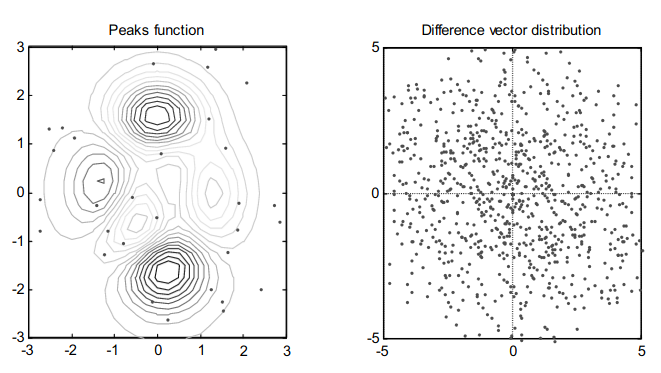
\includegraphics[width=0.8\textwidth,height=0.8\textheight,
    keepaspectratio]{res/cm1.png}
\captionsetup{justification=centering,margin=3cm}
    \caption{Ban đầu, các vector chênh lệch được phân bổ đếu ra mọi hướng.}
  \end{figure}
\end{frame}

\begin{frame}{Contour Matching}
  \begin{figure}
    \centering
    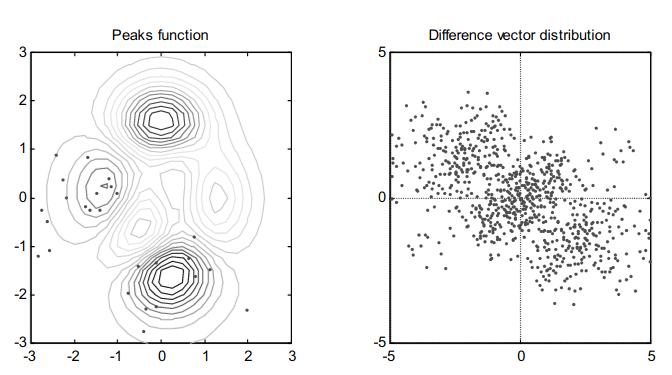
\includegraphics[width=0.8\textwidth,height=0.8\textheight,
    keepaspectratio]{res/cm2.png}
\captionsetup{justification=centering,margin=3cm}
    \caption{Khi các cá thể hội tụ đến hai nghiệm tối ưu địa phương (đỉnh), các vector
    chênh lệch bắt đầu được định hướng.}
  \end{figure}
\end{frame}

\begin{frame}{Contour Matching}
  \begin{figure}
    \centering
    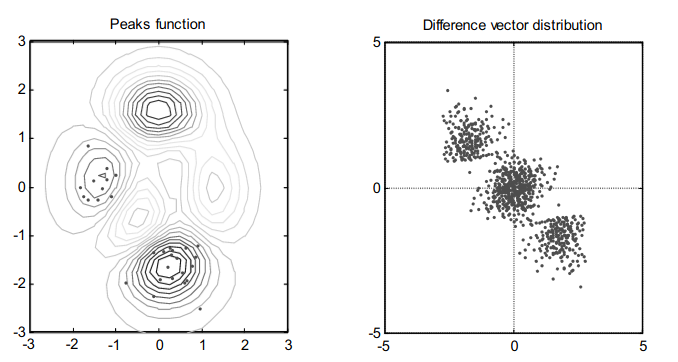
\includegraphics[width=0.8\textwidth,height=0.8\textheight,
    keepaspectratio]{res/cm3.png}
\captionsetup{justification=centering,margin=3cm}
    \caption{Các vector chênh lệch chia thành 3 nhóm: nhóm gần 0, nhóm đi từ
    một đỉnh đến đỉnh còn lại và ngược lại}
  \end{figure}
\end{frame}

\begin{frame}{Contour Matching}
  \begin{figure}
    \centering
    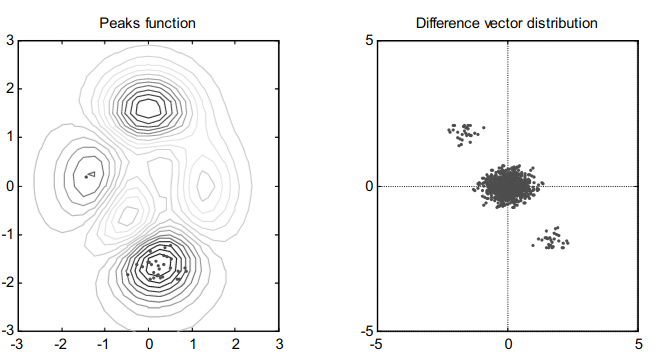
\includegraphics[width=0.8\textwidth,height=0.8\textheight,
    keepaspectratio]{res/cm4.png}
\captionsetup{justification=centering,margin=3cm}
    \caption{Sự phân bố các nhóm trở nên rõ rệt hơn. Mặt khác các cá thể hầu như
    đã hội tụ về một đỉnh, nên nhóm gần 0 đã chiếm đa số}
  \end{figure}
\end{frame}

\begin{frame}{Contour Matching}
  \begin{figure}
    \centering
    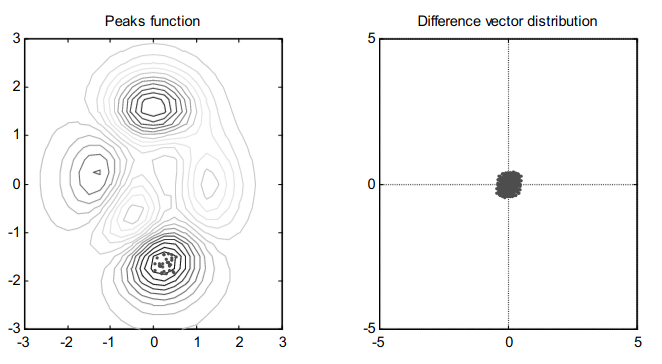
\includegraphics[width=0.8\textwidth,height=0.8\textheight,
    keepaspectratio]{res/cm5.png}
\captionsetup{justification=centering,margin=3cm}
    \caption{Các vector chênh lệch đã hội tụ về gần 0, tất cả các cá thể cũng
      hội tụ về một đỉnh}
  \end{figure}
\end{frame}

\subsection{Ảnh hưởng của các tham số đến DE} % (fold)
\label{sub:Ảnh hưởng của các tham số đến DE}

\begin{frame}{Ảnh hưởng của các tham số đến DE}
Thuật toán DE sử dụng tương đối ít tham số:
\begin{itemize}
\item \( NP \in \mathbb{N} \): số lượng cá thể trong quần thể. Tham số này được
  sử dụng để khởi tạo quần thể, và số lượng cá thể trong quần thể sẽ không đổi
  trong suốt quá trình chạy của thuật toán.
\item \( F \in [0, 2] \): gọi là trọng số vi phân (differential weight). Tham số
  này trực tiếp ảnh hưởng đến quá trình đột biến, là hệ số được nhân vào vector
  chênh lệch trước khi được thêm vào vector cơ sở.
\item \( CR \in [0, 1] \): gọi là tỉ lệ lai ghép (crossover rate). Tham số này
  càng gần 1 thì cá thể con sinh ra sau lai ghép sẽ càng giống với cá thể gốc.
\end{itemize}
\end{frame}

\begin{frame}{Ảnh hưởng của các tham số đến DE}
  \begin{itemize}
  \item 
  \textbf{Chọn} \( NP \): \( NP \) thường được chọn \( NP = 5D \) hoặc \( NP = 10D \), với \( D \) là
  số chiều của bài toán. Trong nghiên cứu của Gamperle \textit{et al.}, giá trị
  \( NP \) nằm giữa \( 3D \) và \( 8D \) sẽ cho ra kết quả tốt nhất.

  Trong thực nghiệm, một giá trị \( NP \) quá lớn cũng sẽ không làm cho thuật
  toán chạy hiệu quả hơn nhiều.

\item \textbf{Chọn} \( F \):
  Mặc dù miền giá trị của \( F \) là \( [0, 2] \), nhưng trong thực nghiệm thì
  \( F \) được chọn trong đoạn nhỏ hơn là \( [0.4, 1] \). Một giá trị hay được
  sử dụng của \( F \) là \( F = 0.5 \).

  Tuy nhiên, nếu \( F \) bàng hoặc gần \( 1 \), thì công thức đột biến nhiều khả
  năng sinh ra một cá thể đã có sẵn, làm mất đi tính đa dạng của quần
  thể. Chính vì thế, K. Price \textit{et al.} cho rằng giá trị \( F \) nên chọn
  trong khoảng \( (0.4, 0.95) \).
\end{itemize}
\end{frame}

\begin{frame}{Ảnh hưởng của các tham số đến DE}
\textbf{Chọn} \( CR \):

  Giá trị \( CR \) cần được chọn tùy thuộc vào hàm mục tiêu. Chú ý rằng khi \(
  CR = 1 \) thì vector cá thể con sẽ chỉ có 1 gen lấy tử cá thể đột biến, nên
  các toán tử đơn giản như DE/rand/1/bin sẽ có tính bất biến theo phép quay:

  \begin{itemize}
  \item Ta chọn \( CR \) là một giá trị thấp (0 hoặc 0.1) nếu như hàm fitness là
    một hàm có tính chất tương đối độc lập đối với từng gen, chẳng hạn như:
    \[
      f(x) = f_{1}(x_{1}) + f_{2}(x_{2}) + \ldots +f_{D}(x_{D})
    .\] 
  \item Nếu trường hợp ngược lại, ta cần chọn \( CR \) là một giá trị lớn hơn.
    Giá trị \( CR \) có thể được chọn trong đoạn \( [0.3, 0.9] \).
  \end{itemize}
\end{frame}

\begin{frame}{Ảnh hưởng của các tham số đến DE}
  Đã có nhiều nghiên cứu về việc cập nhật các tham số \( F \) và \( CR \) trong
  quá trình chạy thuật toán. Những thuật toán này thuộc lớp các thuật toán Adaptive
  Differential Evolution, chẳng hạn như trong SaDE (Self-adaptive Differential
  Evolution), các tham số này được cập nhật như sau:
  \begin{align*}
    F' &= \begin{cases}
      F_{l} + r_{1}(F_{u} - F_{l}), &\text{ nếu } r_{2} < \tau_{1}\\
      F, &\text{ nếu ngược lại }
    \end{cases}\\
      CR' &= \begin{cases}
      r_{3}, &\text{ nếu } r_{4}  < \tau_{2}\\
      CR, &\text{ nếu ngược lại }\\
    \end{cases}
  .\end{align*}

  Các tham số \( F_{l}, F_{u} \)\footnote{Thuật toán gốc lấy \( F_{u} \) là độ
  dài khoảng giá trị của \( F \) (\( F_{u} - F_{l} \)).} là cận dưới
  (\textbf{l}ower bound) và cận trên (\textbf{u}pper bound) của \( F \), \(
  \tau_{1} \) và \( \tau_{2} \) là các
  giá trị xác suất cho hai trường hợp, \( r_{i}, i\in \{1,2 ,3,4\}   \) là các
  số thực ngẫu nhiên giữa \( 0 \) và \( 1 \).
\end{frame}
% subsection Ảnh hưởng của các tham số đến DE (end)

% section Tiến hóa vi phân (Differential Evolution) (end)
